\documentclass{beamer}
\usepackage{beamerthemeuucs}
% \setbeamercovered{transparent} 

\usepackage{amsmath}
\usepackage{amssymb}
\usepackage{amsthm}
\usepackage{bbold} %% Font for fancy math letters
\usepackage{dsfont} %% Font for fancy math letters
\usepackage{scalerel}
\usepackage{graphicx}
% \usepackage{enumitem}
% \usepackage{showframe}

%% Agda stuff
\usepackage[conor]{agda}
\usepackage[draft]{todonotes}
\newcommand{\AK}{\AgdaKeyword}
\newcommand{\AY}{\AgdaSymbol}
\newcommand{\AN}{\AgdaNumber}
\newcommand{\AS}{\AgdaSpace}
\newcommand{\AB}{\AgdaBound}
\newcommand{\AO}{\AgdaOperator}
\newcommand{\AI}{\AgdaInductiveConstructor}
\newcommand{\AC}{\AgdaCoinductiveConstructor}
\newcommand{\AD}{\AgdaDatatype}
\newcommand{\AF}{\AgdaFunction}
\newcommand{\AM}{\AgdaModule}
\newcommand{\AL}{\AgdaField}
\newcommand{\AR}{\AgdaArgument}
\newcommand{\AT}{\AgdaIndent}
\newcommand{\ARR}{\AgdaRecord}
\newcommand{\AP}{\AgdaPostulate}
\newcommand{\APT}{\AgdaPrimitiveType}
\newcommand{\nonterm}[1]{\hspace*{-0.1cm}\colorbox{orange!25}{#1}}
\newcommand{\hole}[1]{\colorbox{yellow!50}{\ensuremath{\bigbox_{#1}}}}

\usepackage{tikz}
\usetikzlibrary{arrows,snakes,backgrounds,calc}
\newcommand{\pgftextcircled}[1]{
    \setbox0=\hbox{#1}%
    \dimen0\wd0%
    \divide\dimen0 by 2%
    \begin{tikzpicture}[baseline=(a.base)]%
        \useasboundingbox (-\the\dimen0,0pt) rectangle (\the\dimen0,1pt);
        \node[circle,draw,outer sep=0pt,inner sep=0.1ex] (a) {\textbf{#1}};
    \end{tikzpicture}
}

%% ODER: format ==         = "\mathrel{==}"
%% ODER: format /=         = "\neq "
%
%
\makeatletter
\@ifundefined{lhs2tex.lhs2tex.sty.read}%
  {\@namedef{lhs2tex.lhs2tex.sty.read}{}%
   \newcommand\SkipToFmtEnd{}%
   \newcommand\EndFmtInput{}%
   \long\def\SkipToFmtEnd#1\EndFmtInput{}%
  }\SkipToFmtEnd

\newcommand\ReadOnlyOnce[1]{\@ifundefined{#1}{\@namedef{#1}{}}\SkipToFmtEnd}
\usepackage{amstext}
\usepackage{amssymb}
\usepackage{stmaryrd}
\DeclareFontFamily{OT1}{cmtex}{}
\DeclareFontShape{OT1}{cmtex}{m}{n}
  {<5><6><7><8>cmtex8
   <9>cmtex9
   <10><10.95><12><14.4><17.28><20.74><24.88>cmtex10}{}
\DeclareFontShape{OT1}{cmtex}{m}{it}
  {<-> ssub * cmtt/m/it}{}
\newcommand{\texfamily}{\fontfamily{cmtex}\selectfont}
\DeclareFontShape{OT1}{cmtt}{bx}{n}
  {<5><6><7><8>cmtt8
   <9>cmbtt9
   <10><10.95><12><14.4><17.28><20.74><24.88>cmbtt10}{}
\DeclareFontShape{OT1}{cmtex}{bx}{n}
  {<-> ssub * cmtt/bx/n}{}
\newcommand{\tex}[1]{\text{\texfamily#1}}	% NEU

\newcommand{\Sp}{\hskip.33334em\relax}


\newcommand{\Conid}[1]{\mathit{#1}}
\newcommand{\Varid}[1]{\mathit{#1}}
\newcommand{\anonymous}{\kern0.06em \vbox{\hrule\@width.5em}}
\newcommand{\plus}{\mathbin{+\!\!\!+}}
\newcommand{\bind}{\mathbin{>\!\!\!>\mkern-6.7mu=}}
\newcommand{\rbind}{\mathbin{=\mkern-6.7mu<\!\!\!<}}% suggested by Neil Mitchell
\newcommand{\sequ}{\mathbin{>\!\!\!>}}
\renewcommand{\leq}{\leqslant}
\renewcommand{\geq}{\geqslant}
\usepackage{polytable}

%mathindent has to be defined
\@ifundefined{mathindent}%
  {\newdimen\mathindent\mathindent\leftmargini}%
  {}%

\def\resethooks{%
  \global\let\SaveRestoreHook\empty
  \global\let\ColumnHook\empty}
\newcommand*{\savecolumns}[1][default]%
  {\g@addto@macro\SaveRestoreHook{\savecolumns[#1]}}
\newcommand*{\restorecolumns}[1][default]%
  {\g@addto@macro\SaveRestoreHook{\restorecolumns[#1]}}
\newcommand*{\aligncolumn}[2]%
  {\g@addto@macro\ColumnHook{\column{#1}{#2}}}

\resethooks

\newcommand{\onelinecommentchars}{\quad-{}- }
\newcommand{\commentbeginchars}{\enskip\{-}
\newcommand{\commentendchars}{-\}\enskip}

\newcommand{\visiblecomments}{%
  \let\onelinecomment=\onelinecommentchars
  \let\commentbegin=\commentbeginchars
  \let\commentend=\commentendchars}

\newcommand{\invisiblecomments}{%
  \let\onelinecomment=\empty
  \let\commentbegin=\empty
  \let\commentend=\empty}

\visiblecomments

\newlength{\blanklineskip}
\setlength{\blanklineskip}{0.66084ex}

\newcommand{\hsindent}[1]{\quad}% default is fixed indentation
\let\hspre\empty
\let\hspost\empty
\newcommand{\NB}{\textbf{NB}}
\newcommand{\Todo}[1]{$\langle$\textbf{To do:}~#1$\rangle$}

\EndFmtInput
\makeatother
%
%
%
%
%
%
% This package provides two environments suitable to take the place
% of hscode, called "plainhscode" and "arrayhscode". 
%
% The plain environment surrounds each code block by vertical space,
% and it uses \abovedisplayskip and \belowdisplayskip to get spacing
% similar to formulas. Note that if these dimensions are changed,
% the spacing around displayed math formulas changes as well.
% All code is indented using \leftskip.
%
% Changed 19.08.2004 to reflect changes in colorcode. Should work with
% CodeGroup.sty.
%
\ReadOnlyOnce{polycode.fmt}%
\makeatletter

\newcommand{\hsnewpar}[1]%
  {{\parskip=0pt\parindent=0pt\par\vskip #1\noindent}}

% can be used, for instance, to redefine the code size, by setting the
% command to \small or something alike
\newcommand{\hscodestyle}{}

% The command \sethscode can be used to switch the code formatting
% behaviour by mapping the hscode environment in the subst directive
% to a new LaTeX environment.

\newcommand{\sethscode}[1]%
  {\expandafter\let\expandafter\hscode\csname #1\endcsname
   \expandafter\let\expandafter\endhscode\csname end#1\endcsname}

% "compatibility" mode restores the non-polycode.fmt layout.

\newenvironment{compathscode}%
  {\par\noindent
   \advance\leftskip\mathindent
   \hscodestyle
   \let\\=\@normalcr
   \let\hspre\(\let\hspost\)%
   \pboxed}%
  {\endpboxed\)%
   \par\noindent
   \ignorespacesafterend}

\newcommand{\compaths}{\sethscode{compathscode}}

% "plain" mode is the proposed default.
% It should now work with \centering.
% This required some changes. The old version
% is still available for reference as oldplainhscode.

\newenvironment{plainhscode}%
  {\hsnewpar\abovedisplayskip
   \advance\leftskip\mathindent
   \hscodestyle
   \let\hspre\(\let\hspost\)%
   \pboxed}%
  {\endpboxed%
   \hsnewpar\belowdisplayskip
   \ignorespacesafterend}

\newenvironment{oldplainhscode}%
  {\hsnewpar\abovedisplayskip
   \advance\leftskip\mathindent
   \hscodestyle
   \let\\=\@normalcr
   \(\pboxed}%
  {\endpboxed\)%
   \hsnewpar\belowdisplayskip
   \ignorespacesafterend}

% Here, we make plainhscode the default environment.

\newcommand{\plainhs}{\sethscode{plainhscode}}
\newcommand{\oldplainhs}{\sethscode{oldplainhscode}}
\plainhs

% The arrayhscode is like plain, but makes use of polytable's
% parray environment which disallows page breaks in code blocks.

\newenvironment{arrayhscode}%
  {\hsnewpar\abovedisplayskip
   \advance\leftskip\mathindent
   \hscodestyle
   \let\\=\@normalcr
   \(\parray}%
  {\endparray\)%
   \hsnewpar\belowdisplayskip
   \ignorespacesafterend}

\newcommand{\arrayhs}{\sethscode{arrayhscode}}

% The mathhscode environment also makes use of polytable's parray 
% environment. It is supposed to be used only inside math mode 
% (I used it to typeset the type rules in my thesis).

\newenvironment{mathhscode}%
  {\parray}{\endparray}

\newcommand{\mathhs}{\sethscode{mathhscode}}

% texths is similar to mathhs, but works in text mode.

\newenvironment{texthscode}%
  {\(\parray}{\endparray\)}

\newcommand{\texths}{\sethscode{texthscode}}

% The framed environment places code in a framed box.

\def\codeframewidth{\arrayrulewidth}
\RequirePackage{calc}

\newenvironment{framedhscode}%
  {\parskip=\abovedisplayskip\par\noindent
   \hscodestyle
   \arrayrulewidth=\codeframewidth
   \tabular{@{}|p{\linewidth-2\arraycolsep-2\arrayrulewidth-2pt}|@{}}%
   \hline\framedhslinecorrect\\{-1.5ex}%
   \let\endoflinesave=\\
   \let\\=\@normalcr
   \(\pboxed}%
  {\endpboxed\)%
   \framedhslinecorrect\endoflinesave{.5ex}\hline
   \endtabular
   \parskip=\belowdisplayskip\par\noindent
   \ignorespacesafterend}

\newcommand{\framedhslinecorrect}[2]%
  {#1[#2]}

\newcommand{\framedhs}{\sethscode{framedhscode}}

% The inlinehscode environment is an experimental environment
% that can be used to typeset displayed code inline.

\newenvironment{inlinehscode}%
  {\(\def\column##1##2{}%
   \let\>\undefined\let\<\undefined\let\\\undefined
   \newcommand\>[1][]{}\newcommand\<[1][]{}\newcommand\\[1][]{}%
   \def\fromto##1##2##3{##3}%
   \def\nextline{}}{\) }%

\newcommand{\inlinehs}{\sethscode{inlinehscode}}

% The joincode environment is a separate environment that
% can be used to surround and thereby connect multiple code
% blocks.

\newenvironment{joincode}%
  {\let\orighscode=\hscode
   \let\origendhscode=\endhscode
   \def\endhscode{\def\hscode{\endgroup\def\@currenvir{hscode}\\}\begingroup}
   %\let\SaveRestoreHook=\empty
   %\let\ColumnHook=\empty
   %\let\resethooks=\empty
   \orighscode\def\hscode{\endgroup\def\@currenvir{hscode}}}%
  {\origendhscode
   \global\let\hscode=\orighscode
   \global\let\endhscode=\origendhscode}%

\makeatother
\EndFmtInput
%

%% Agda keywords

%% Agda standard types

%% Constructors of the above types

%% Some standard functions
% format map    = "\AF{map}"       % Disabled

%% Non-colored stuff

%% Useful symbols


\renewcommand\hscodestyle{%
   \setlength\leftskip{0.1cm}%
   \small
}
\title{From Algebra to Abstract Machine:\\ A Verified Generic Construction}
\subtitle{TyDe'18}
\author{\underline{Carlos Tomé Cortiñas}* and Wouter Swierstra}
\date{September 2018\\
% \vspace{2em}

\flushleft
\textbf{*} Sponsored by

\hspace{3em}
\includegraphics[angle=90, scale=0.15]{img/logo_ufonds.pdf}

}


\begin{document}
\frame{\titlepage}

% Datatypes


% Constructors

% Functions





% Bound variables



%Numbers



\frame{
  \frametitle{To put it another way ...}
  \begin{center}
    {\Large Verified tail-recursive folds through dissection}
  \end{center}
}

\section{Motivation}

\frame{
  \frametitle{Motivation}

  We start with a small \ensuremath{\AD{Expr}}ession language

  \pause

  \begin{hscode}\SaveRestoreHook
\column{B}{@{}>{\hspre}l<{\hspost}@{}}%
\column{3}{@{}>{\hspre}l<{\hspost}@{}}%
\column{5}{@{}>{\hspre}l<{\hspost}@{}}%
\column{10}{@{}>{\hspre}l<{\hspost}@{}}%
\column{13}{@{}>{\hspre}l<{\hspost}@{}}%
\column{19}{@{}>{\hspre}l<{\hspost}@{}}%
\column{E}{@{}>{\hspre}l<{\hspost}@{}}%
\>[3]{}\AK{data}\;\AD{Expr}\;\mathbin{:}\;\AP{Set}\;\AK{where}{}\<[E]%
\\
\>[3]{}\hsindent{2}{}\<[5]%
\>[5]{}\AI{Val}\;{}\<[10]%
\>[10]{}\mathbin{:}\;{}\<[13]%
\>[13]{}\AD{\ensuremath{\mathbb{N}}}\;{}\<[19]%
\>[19]{}\to \;\AD{Expr}{}\<[E]%
\\
\>[3]{}\hsindent{2}{}\<[5]%
\>[5]{}\AI{Add}\;{}\<[10]%
\>[10]{}\mathbin{:}\;{}\<[13]%
\>[13]{}\AD{Expr}\;{}\<[19]%
\>[19]{}\to \;\AD{Expr}\;\to \;\AD{Expr}{}\<[E]%
\ColumnHook
\end{hscode}\resethooks

  \pause

  and we write an \ensuremath{\AF{eval}}uator for it.

  \pause

  \begin{hscode}\SaveRestoreHook
\column{B}{@{}>{\hspre}l<{\hspost}@{}}%
\column{3}{@{}>{\hspre}l<{\hspost}@{}}%
\column{21}{@{}>{\hspre}l<{\hspost}@{}}%
\column{E}{@{}>{\hspre}l<{\hspost}@{}}%
\>[3]{}\AF{eval}\;\mathbin{:}\;\AD{Expr}\;\to \;\AD{\ensuremath{\mathbb{N}}}{}\<[E]%
\\
\>[3]{}\AF{eval}\;(\AI{Val}\;\AB{n})\;{}\<[21]%
\>[21]{}\mathrel{=}\;\AB{n}{}\<[E]%
\\
\>[3]{}\AF{eval}\;(\AI{Add}\;\AB{\ensuremath{e_1}}\;\AB{\ensuremath{e_2}})\;{}\<[21]%
\>[21]{}\mathrel{=}\;\AF{eval}\;\AB{\ensuremath{e_1}}\;\AF{+}\;\AF{eval}\;\AB{\ensuremath{e_2}}{}\<[E]%
\ColumnHook
\end{hscode}\resethooks
}


\frame{
  \frametitle{A Problem with \ensuremath{\AF{eval}}}

  \begin{hscode}\SaveRestoreHook
\column{B}{@{}>{\hspre}l<{\hspost}@{}}%
\column{5}{@{}>{\hspre}l<{\hspost}@{}}%
\column{E}{@{}>{\hspre}l<{\hspost}@{}}%
\>[5]{}\Varid{>}\;\AF{eval}\;(\AI{Add}\;(\AI{Add}\;(\AI{Add}\;\Varid{...}\;(\AI{Add}\;(\AI{Val}\;\AN{1})\;(\AI{Val}\;\AN{2})))))\mbox{\onelinecomment  large expression}{}\<[E]%
\ColumnHook
\end{hscode}\resethooks
  \pause
  \vspace*{-1cm}
  \begin{hscode}\SaveRestoreHook
\column{B}{@{}>{\hspre}l<{\hspost}@{}}%
\column{5}{@{}>{\hspre}l<{\hspost}@{}}%
\column{E}{@{}>{\hspre}l<{\hspost}@{}}%
\>[5]{}\Varid{***}\;\Conid{Exception:}\;\Varid{stack}\;\Varid{overflow}{}\<[E]%
\ColumnHook
\end{hscode}\resethooks

  \pause

  What happened? \pause A \textbf{well-typed} program \textit{went wrong}.

  \pause

  \begin{itemize}[<+->]
    \setlength\itemsep{1em}
    \item \ensuremath{\AF{eval}} evaluates  \underline{both} subtrees before reducing \ensuremath{\AF{\_+\_}}
      further.
    \item Record unevaluated subtrees on the stack.
    \item On large inputs, the \textbf{stack} might \textbf{overflow}.
  \end{itemize}
}

\frame{
  \frametitle{A solution to the problem}

  \pause
  \begin{center}
    \Large{Write a \textbf{tail-recursive} evaluator.}
  \end{center}

  \pause
  We proceed in \textit{three steps}:

  \pause

  \begin{itemize}[<+->]
    \setlength\itemsep{1em}
    \item Make the underlying stack \underline{explicit}.
    \item Define a \textit{tail-recursive} function over the stack.
    \item Show that it is equivalent to \ensuremath{\AF{eval}}.
  \end{itemize}
}


\frame{
  \frametitle{A tail-recursive evaluator}

  \begin{hscode}\SaveRestoreHook
\column{B}{@{}>{\hspre}l<{\hspost}@{}}%
\column{5}{@{}>{\hspre}l<{\hspost}@{}}%
\column{7}{@{}>{\hspre}l<{\hspost}@{}}%
\column{14}{@{}>{\hspre}l<{\hspost}@{}}%
\column{22}{@{}>{\hspre}l<{\hspost}@{}}%
\column{E}{@{}>{\hspre}l<{\hspost}@{}}%
\>[5]{}\AK{data}\;\AD{Stack}\;\mathbin{:}\;\AP{Set}\;\AK{where}{}\<[E]%
\\
\>[5]{}\hsindent{2}{}\<[7]%
\>[7]{}\AI{Top}\;{}\<[14]%
\>[14]{}\mathbin{:}\;\AD{Stack}{}\<[E]%
\\
\>[5]{}\hsindent{2}{}\<[7]%
\>[7]{}\AI{Left}\;{}\<[14]%
\>[14]{}\mathbin{:}\;\AD{Expr}\;{}\<[22]%
\>[22]{}\to \;\AD{Stack}\;\to \;\AD{Stack}{}\<[E]%
\\
\>[5]{}\hsindent{2}{}\<[7]%
\>[7]{}\AI{Right}\;{}\<[14]%
\>[14]{}\mathbin{:}\;\AD{\ensuremath{\mathbb{N}}}\;{}\<[22]%
\>[22]{}\to \;\AD{Stack}\;\to \;\AD{Stack}{}\<[E]%
\ColumnHook
\end{hscode}\resethooks

  \pause
  \vspace*{-0.5cm}
  \begin{hscode}\SaveRestoreHook
\column{B}{@{}>{\hspre}l<{\hspost}@{}}%
\column{3}{@{}>{\hspre}l<{\hspost}@{}}%
\column{5}{@{}>{\hspre}l<{\hspost}@{}}%
\column{17}{@{}>{\hspre}l<{\hspost}@{}}%
\column{23}{@{}>{\hspre}l<{\hspost}@{}}%
\column{33}{@{}>{\hspre}l<{\hspost}@{}}%
\column{E}{@{}>{\hspre}l<{\hspost}@{}}%
\>[3]{}\AK{mutual}{}\<[E]%
\\
\>[3]{}\hsindent{2}{}\<[5]%
\>[5]{}\AF{load}\;\mathbin{:}\;\AD{Expr}\;\to \;\AD{Stack}\;\to \;\AD{\ensuremath{\mathbb{N}}}{}\<[E]%
\\
\>[3]{}\hsindent{2}{}\<[5]%
\>[5]{}\AF{load}\;(\AI{Val}\;\AB{n})\;{}\<[23]%
\>[23]{}\AB{stk}\;\mathrel{=}\;\AF{unload}\;\AB{n}\;\AB{stk}{}\<[E]%
\\
\>[3]{}\hsindent{2}{}\<[5]%
\>[5]{}\AF{load}\;(\AI{Add}\;\AB{\ensuremath{e_1}}\;\AB{\ensuremath{e_2}})\;{}\<[23]%
\>[23]{}\AB{stk}\;\mathrel{=}\;\AF{load}\;\AB{\ensuremath{e_1}}\;(\AI{Left}\;\AB{\ensuremath{e_2}}\;\AB{stk}){}\<[E]%
\\[\blanklineskip]%
\>[3]{}\hsindent{2}{}\<[5]%
\>[5]{}\AF{unload}\;\mathbin{:}\;\AD{\ensuremath{\mathbb{N}}}\;\to \;\AD{Stack}\;\to \;\AD{\ensuremath{\mathbb{N}}}{}\<[E]%
\\
\>[3]{}\hsindent{2}{}\<[5]%
\>[5]{}\AF{unload}\;\AB{v}\;{}\<[17]%
\>[17]{}\AI{Top}\;{}\<[33]%
\>[33]{}\mathrel{=}\;\AB{v}{}\<[E]%
\\
\>[3]{}\hsindent{2}{}\<[5]%
\>[5]{}\AF{unload}\;\AB{v}\;{}\<[17]%
\>[17]{}(\AI{Left}\;\AB{e}\;\AB{stk})\;{}\<[33]%
\>[33]{}\mathrel{=}\;\AF{load}\;\AB{e}\;(\AI{Right}\;\AB{v}\;\AB{stk}){}\<[E]%
\\
\>[3]{}\hsindent{2}{}\<[5]%
\>[5]{}\AF{unload}\;\AB{v}\;{}\<[17]%
\>[17]{}(\AI{Right}\;\AB{v'}\;\AB{stk})\;{}\<[33]%
\>[33]{}\mathrel{=}\;\AF{unload}\;(\AB{v'}\;\AF{+}\;\AB{v})\;\AB{stk}{}\<[E]%
\ColumnHook
\end{hscode}\resethooks
  \pause
  \vspace*{-1cm}
  \begin{hscode}\SaveRestoreHook
\column{B}{@{}>{\hspre}l<{\hspost}@{}}%
\column{3}{@{}>{\hspre}l<{\hspost}@{}}%
\column{E}{@{}>{\hspre}l<{\hspost}@{}}%
\>[3]{}\AF{tail\text{-}rec\text{-}eval}\;\mathbin{:}\;\AD{Expr}\;\to \;\AD{\ensuremath{\mathbb{N}}}{}\<[E]%
\\
\>[3]{}\AF{tail\text{-}rec\text{-}eval}\;\AB{e}\;\mathrel{=}\;\AF{load}\;\AB{e}\;\AI{Top}{}\<[E]%
\ColumnHook
\end{hscode}\resethooks
}


\frame {
  \frametitle{\ensuremath{\AF{tail\text{-}rec\text{-}eval}} in action}

  \begin{center}
    \only<1>{\Large\ensuremath{\AF{load}\;(\AI{Add}\;(\AI{Val}\;\AN{1})\;(\AI{Add}\;(\AI{Val}\;\AN{2})\;(\AI{Val}\;\AN{2})))\;\underline{\AI{Top}}}}
    \only<2>{\Large\ensuremath{\AF{load}\;(\AI{Val}\;\AN{1})\;(\underline{\AI{Left}}\;(\AI{Add}\;(\AI{Val}\;\AN{2})\;(\AI{Val}\;\AN{2}))\;\underline{\AI{Top}})}}
    \only<3>{\Large\ensuremath{\AF{unload}\;\AN{1}\;(\underline{\AI{Left}}\;(\AI{Add}\;(\AI{Val}\;\AN{2})\;(\AI{Val}\;\AN{2}))\;\underline{\AI{Top}})}}
    \only<4>{\Large\ensuremath{\AF{load}\;(\AI{Add}\;(\AI{Val}\;\AN{2})\;(\AI{Val}\;\AN{2}))\;(\underline{\AI{Right}}\;\AN{1}\;\underline{\AI{Top}})}}
    \only<5>{\Large\ensuremath{\AF{load}\;(\AI{Val}\;\AN{2})\;(\underline{\AI{Left}}\;(\AI{Val}\;\AN{2})\;(\underline{\AI{Right}}\;\AN{1}\;\underline{\AI{Top}}))}}
    \only<6>{\Large\ensuremath{\AF{unload}\;\AN{2}\;(\underline{\AI{Left}}\;(\AI{Val}\;\AN{2})\;(\underline{\AI{Right}}\;\AN{1}\;\underline{\AI{Top}}))}}
    \only<7>{\Large\ensuremath{\AF{load}\;(\AI{Val}\;\AN{2})\;(\underline{\AI{Right}}\;\AN{2}\;(\underline{\AI{Right}}\;\AN{1}\;\underline{\AI{Top}}))}}
    \only<8>{\Large\ensuremath{\AF{unload}\;\AN{2}\;(\underline{\AI{Right}}\;\AN{2}\;(\underline{\AI{Right}}\;\AN{1}\;\underline{\AI{Top}}))}}
    \only<9>{\Large\ensuremath{\AF{unload}\;(\AN{2}\;\AF{+}\;\AN{2})\;(\underline{\AI{Right}}\;\AN{1}\;\underline{\AI{Top}})}}
    \only<10>{\Large\ensuremath{\AF{unload}\;\AN{4}\;(\underline{\AI{Right}}\;\AN{1}\;\underline{\AI{Top}})}}
    \only<11>{\Large\ensuremath{\AF{unload}\;(\AN{1}\;\AF{+}\;\AN{4})\;\underline{\AI{Top}}}}
    \only<12>{\Large\ensuremath{\AF{unload}\;\AN{5}\;\underline{\AI{Top}}}}

    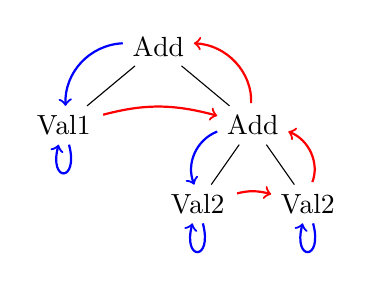
\begin{tikzpicture}
  % \tikzstyle{every node}=[font=\footnotesize]
  \tikzstyle{level 1}=[level distance=10mm, sibling distance=24mm]
  \tikzstyle{level 2}=[level distance=10mm, sibling distance=14mm]
  \tikzstyle{level 3}=[level distance=10mm, sibling distance=14mm]
  \tikzstyle{load}=[->,thick,color=blue]
  \tikzstyle{unload}=[->,shorten <=1pt,thick,color=red]

  \node (root) {\AI{Add}}
    child {node (node1) {\AI{Val}\AS{}\AN{1}}} 
    child {node (node2) {\AI{Add}} 
           child {node (node3) {\AI{Val}\AS{}\AN{2}}}
           child {node (node4) {\AI{Val}\AS{}\AN{2}}}};


  \onslide<2->{\draw[load] (root) to [ bend right=45] (node1);}
  \onslide<3->{\draw[load] (node1) to [ loop below ] (node1);}
  \onslide<4->{\draw[unload] (node1) to [ bend left=15] (node2);}
  \onslide<5->{\draw[load] (node2) to [ bend right=45] (node3);}
  \onslide<6->{\draw[load] (node3) to [ loop below] (node3);}
  \onslide<7->{\draw[unload] (node3) to [ bend left=15] (node4);}
  \onslide<8->{\draw[load] (node4) to [ loop below] (node4);}
  \onslide<9->{\draw[unload] (node4) to [ bend right=45] (node2);}
  \onslide<11->{\draw[unload] (node2) to [ bend right=45] (root);}
\end{tikzpicture}

  \end{center}
}

\frame{
  \frametitle{Problem solved?}

  \begin{center}
    {\large Have we \textbf{actually} solved the problem?}
  \end{center}

  \pause

  Is \textbf{really} \ensuremath{\AF{tail\text{-}rec\text{-}eval}} \textit{equivalent} to \ensuremath{\AF{eval}}? \pause Can we \underline{prove} it?

  \pause

  \begin{hscode}\SaveRestoreHook
\column{B}{@{}>{\hspre}l<{\hspost}@{}}%
\column{5}{@{}>{\hspre}l<{\hspost}@{}}%
\column{7}{@{}>{\hspre}l<{\hspost}@{}}%
\column{19}{@{}>{\hspre}l<{\hspost}@{}}%
\column{35}{@{}>{\hspre}l<{\hspost}@{}}%
\column{E}{@{}>{\hspre}l<{\hspost}@{}}%
\>[5]{}\AK{mutual}{}\<[E]%
\\
\>[5]{}\hsindent{2}{}\<[7]%
\>[7]{}\nonterm{\AF{load}}\;\mathbin{:}\;\AD{Expr}\;\to \;\AD{Stack}\;\to \;\AD{\ensuremath{\mathbb{N}}}{}\<[E]%
\\
\>[5]{}\hsindent{2}{}\<[7]%
\>[7]{}\Varid{...}{}\<[E]%
\\[\blanklineskip]%
\>[5]{}\hsindent{2}{}\<[7]%
\>[7]{}\nonterm{\AF{unload}}\;\mathbin{:}\;\AD{\ensuremath{\mathbb{N}}}\;\to \;\AD{Stack}\;\to \;\AD{\ensuremath{\mathbb{N}}}{}\<[E]%
\\
\>[5]{}\hsindent{2}{}\<[7]%
\>[7]{}\AF{unload}\;\AB{v}\;{}\<[19]%
\>[19]{}\AI{Top}\;{}\<[35]%
\>[35]{}\mathrel{=}\;\AB{v}{}\<[E]%
\\
\>[5]{}\hsindent{2}{}\<[7]%
\>[7]{}\AF{unload}\;\AB{v}\;{}\<[19]%
\>[19]{}(\AI{Left}\;\AB{e}\;\AB{stk})\;{}\<[35]%
\>[35]{}\mathrel{=}\;\nonterm{\AF{load}}\;\AB{e}\;(\AI{Right}\;\AB{v}\;\AB{stk}){}\<[E]%
\\
\>[5]{}\hsindent{2}{}\<[7]%
\>[7]{}\AF{unload}\;\AB{v}\;{}\<[19]%
\>[19]{}(\AI{Right}\;\AB{v'}\;\AB{stk})\;{}\<[35]%
\>[35]{}\mathrel{=}\;\nonterm{\AF{unload}}\;(\AB{v'}\;\AF{+}\;\AB{v})\;\AB{stk}{}\<[E]%
\ColumnHook
\end{hscode}\resethooks

  \pause

  We \textbf{lost} termination guarantees.
}

\section{Contributions}

\frame{
  \frametitle{Contributions}
  \begin{itemize}[<+->]
    \setlength\itemsep{2em}
    \item[\textbf{Termination}] We \textbf{construct} a tail-recursive evaluator that terminates
        for every input.
    \item[\textbf{Correctness}] We \textbf{prove} it equal to the original \ensuremath{\AF{eval}} function.
    \item[\textbf{Generalization}]<0> We generalize our result to any
      \textit{catamorphism} and any \textit{algebra} over any \textbf{regular} datatype.
  \end{itemize}
}

\frame{
  \frametitle{That's not all}
  \ensuremath{\AF{eval}} is an example of a \textit{fold} over the \ensuremath{\AD{Expr}} datatype.

  \pause

  \begin{hscode}\SaveRestoreHook
\column{B}{@{}>{\hspre}l<{\hspost}@{}}%
\column{5}{@{}>{\hspre}l<{\hspost}@{}}%
\column{37}{@{}>{\hspre}l<{\hspost}@{}}%
\column{E}{@{}>{\hspre}l<{\hspost}@{}}%
\>[5]{}\AF{fold}\;\mathbin{:}\;(\AB{\ensuremath{\alpha}}\;\to \;\AB{\ensuremath{\alpha}}\;\to \;\AB{\ensuremath{\alpha}})\;\to \;(\AD{\ensuremath{\mathbb{N}}}\;\to \;\AB{\ensuremath{\alpha}})\;\to \;\AD{Expr}\;\to \;\AD{\ensuremath{\mathbb{N}}}{}\<[E]%
\\
\>[5]{}\AF{fold}\;\AB{\ensuremath{\phi_1}}\;\AB{\ensuremath{\phi_2}}\;(\AI{Val}\;\AB{n})\;{}\<[37]%
\>[37]{}\mathrel{=}\;\AB{\ensuremath{\phi_2}}\;\AB{n}{}\<[E]%
\\
\>[5]{}\AF{fold}\;\AB{\ensuremath{\phi_1}}\;\AB{\ensuremath{\phi_2}}\;(\AI{Add}\;\AB{\ensuremath{e_1}}\;\AB{\ensuremath{e_2}})\;{}\<[37]%
\>[37]{}\mathrel{=}\;\AB{\ensuremath{\phi_1}}\;(\AF{fold}\;\AB{\ensuremath{\phi_1}}\;\AB{\ensuremath{\phi_2}}\;\AB{\ensuremath{e_1}})\;(\AF{fold}\;\AB{\ensuremath{\phi_1}}\;\AB{\ensuremath{\phi_2}}\;\AB{\ensuremath{e_2}}){}\<[E]%
\ColumnHook
\end{hscode}\resethooks

  \pause

  Both versions of the function are \underline{the same}.

  \pause

  \begin{hscode}\SaveRestoreHook
\column{B}{@{}>{\hspre}l<{\hspost}@{}}%
\column{5}{@{}>{\hspre}l<{\hspost}@{}}%
\column{E}{@{}>{\hspre}l<{\hspost}@{}}%
\>[5]{}\forall\;(\AB{e}\;\mathbin{:}\;\AD{Expr})\;\to \;\AF{eval}\;\AB{e}\;\AD{\ensuremath{\equiv}}\;\AF{fold}\;\AF{\_+\_}\;\AF{id}\;\AB{e}{}\<[E]%
\ColumnHook
\end{hscode}\resethooks

  \pause

  Moreover:

  \pause

  \begin{itemize}[<+->]
     \item \ensuremath{\AD{Expr}} is an example of a \textbf{regular} type.
     \item \ensuremath{\AF{fold}} is an instance of a \textbf{catamorphism}.
  \end{itemize}
}

\frame{
  \frametitle{Contributions}
  \hspace{3em\hspace{3em}}\begin{itemize}
    \setlength\itemsep{2em}
    \item[\textbf{Termination}] We \textbf{construct} a tail-recursive evaluator that terminates
        for every input.
    \item[\textbf{Correctness}] We \textbf{prove} it equal to the original \ensuremath{\AF{eval}} function.
    \pause
    \item[\textbf{Generalization}] We generalize our result to any
      \textit{catamorphism} and any \textit{algebra} over any \textbf{regular} datatype.
  \end{itemize}

  \pause

  \hspace{1em}\Large{Everything is machine-checked by \textit{Agda}}.
}


\section{Solving the problem}

\frame{
  \frametitle{Plan of attack}
  \begin{enumerate}[<+->]
    \setlength\itemsep{1em}
    \item Break down the \ensuremath{\AK{mutual}} recursion in \ensuremath{\AF{load}} and \ensuremath{\AF{unload}}.
    \item Use \ensuremath{\AF{unload\ensuremath{^{+}}}} to iterate through an \ensuremath{\AD{Expr}} to get a value.
    \item Show that \ensuremath{\AF{unload\ensuremath{^{+}}}} delivers something ``smaller``, thus the iteration
      terminates.
    \item Prove that the resulting function is equivalent to \ensuremath{\AF{eval}}.
  \end{enumerate}
}

\frame{
  \frametitle{Breaking down mutual recursion}

 \begin{hscode}\SaveRestoreHook
\column{B}{@{}>{\hspre}l<{\hspost}@{}}%
\column{4}{@{}>{\hspre}l<{\hspost}@{}}%
\column{17}{@{}>{\hspre}l<{\hspost}@{}}%
\column{31}{@{}>{\hspre}l<{\hspost}@{}}%
\column{34}{@{}>{\hspre}l<{\hspost}@{}}%
\column{E}{@{}>{\hspre}l<{\hspost}@{}}%
\>[4]{}\AF{unload\ensuremath{^{+}}}\;\mathbin{:}\;(\AD{\ensuremath{\mathbb{N}}}\;\AF{\ensuremath{\times}}\;\AD{Stack})\;\to \;(\AD{\ensuremath{\mathbb{N}}}\;\AF{\ensuremath{\times}}\;\AD{Stack})\;\AD{\ensuremath{\uplus}}\;\AD{\ensuremath{\mathbb{N}}}{}\<[E]%
\\
\>[4]{}\AF{unload\ensuremath{^{+}}}\;(\AB{v}\;\Varid{,}\;{}\<[17]%
\>[17]{}\AI{Top}{}\<[31]%
\>[31]{})\;{}\<[34]%
\>[34]{}\mathrel{=}\;\AI{inj\ensuremath{_2}}\;\AB{v}{}\<[E]%
\\
\>[4]{}\AF{unload\ensuremath{^{+}}}\;(\AB{v}\;\Varid{,}\;{}\<[17]%
\>[17]{}\AI{Right}\;\AB{v'}\;\AB{stk}{}\<[31]%
\>[31]{})\;{}\<[34]%
\>[34]{}\mathrel{=}\;\AF{unload\ensuremath{^{+}}}\;(\AB{v'}\;\AF{+}\;\AB{v}\;\Varid{,}\;\AB{stk}){}\<[E]%
\\
\>[4]{}\AF{unload\ensuremath{^{+}}}\;(\AB{v}\;\Varid{,}\;{}\<[17]%
\>[17]{}\AI{Left}\;\AB{e}\;\AB{stk}{}\<[31]%
\>[31]{})\;{}\<[34]%
\>[34]{}\mathrel{=}\;\AF{load}\;\AB{e}\;(\AI{Right}\;\AB{v}\;\AB{stk}){}\<[E]%
\ColumnHook
\end{hscode}\resethooks

 \pause

 \begin{hscode}\SaveRestoreHook
\column{B}{@{}>{\hspre}l<{\hspost}@{}}%
\column{4}{@{}>{\hspre}l<{\hspost}@{}}%
\column{22}{@{}>{\hspre}l<{\hspost}@{}}%
\column{E}{@{}>{\hspre}l<{\hspost}@{}}%
\>[4]{}\AF{load}\;\mathbin{:}\;\AD{Expr}\;\to \;\AD{Stack}\;\to \;(\AD{\ensuremath{\mathbb{N}}}\;\AF{\ensuremath{\times}}\;\AD{Stack})\;\AD{\ensuremath{\uplus}}\;\AD{\ensuremath{\mathbb{N}}}{}\<[E]%
\\
\>[4]{}\AF{load}\;(\AI{Val}\;\AB{n})\;{}\<[22]%
\>[22]{}\AB{stk}\;\mathrel{=}\;\AI{inj\ensuremath{_1}}\;(\AB{n}\;\Varid{,}\;\AB{stk}){}\<[E]%
\\
\>[4]{}\AF{load}\;(\AI{Add}\;\AB{\ensuremath{e_1}}\;\AB{\ensuremath{e_2}})\;{}\<[22]%
\>[22]{}\AB{stk}\;\mathrel{=}\;\AF{load}\;\AB{\ensuremath{e_1}}\;(\AI{Left}\;\AB{\ensuremath{e_2}}\;\AB{stk}){}\<[E]%
\ColumnHook
\end{hscode}\resethooks

 \pause
 Now, both functions \emph{obviously} terminate.
}


\frame{
  \frametitle{A step back}

  \begin{center}
    {\large \ensuremath{\AF{unload\ensuremath{^{+}}}\;\mathbin{:}\;(\AD{\ensuremath{\mathbb{N}}}\;\AF{\ensuremath{\times}}\;\AD{Stack})\;\to \;(\AD{\ensuremath{\mathbb{N}}}\;\AF{\ensuremath{\times}}\;\AD{Stack})\;\AD{\ensuremath{\uplus}}\;\AD{\ensuremath{\mathbb{N}}}}}
  \end{center}
  \pause
  \begin{itemize}[<+->]
    \setlength\itemsep{1em}
    \item \ensuremath{\AF{unload\ensuremath{^{+}}}} is the ``step`` function of an \underline{abstract machine}!

    \item Configurations: \ensuremath{\AD{Config}\;\mathrel{=}\;\AD{\ensuremath{\mathbb{N}}}\;\AF{\ensuremath{\times}}\;\AD{Stack}}

    \item Step function: \ensuremath{\AF{unload\ensuremath{^{+}}}\;\mathbin{:}\;\AD{Config}\;\to \;\AD{Config}\;\AD{\ensuremath{\uplus}}\;\AD{\ensuremath{\mathbb{N}}}}
  \end{itemize}
}

\frame{
  \frametitle{Well-founded recursion}
    \begin{itemize}[<+->]
    \setlength\itemsep{1em}
      \item \ensuremath{\Varid{f}\;\mathbin{:}\;\AB{\ensuremath{\alpha}}\;\to \;\AB{\ensuremath{\alpha}}} \textbf{not} defined by structural recursion.
      \item A relation \ensuremath{\AD{\ensuremath{\_<\_}}\;\mathbin{:}\;\AB{\ensuremath{\alpha}}\;\to \;\AB{\ensuremath{\alpha}}\;\to \;\AP{Set}} such that \ensuremath{\Varid{f}\;\AB{\ensuremath{\alpha}}\;\AD{<}\;\AB{\ensuremath{\alpha}}}.
      \item No infinitely long \textbf{decreasing chains}\\
        \hspace*{5em} $\Longrightarrow$ recursion eventually
        \underline{terminates}.
      \item In \textit{Agda} we encode such property as an accessibility
        predicate.
      \item A relation is \textbf{well-founded} if every element is accessible.
    \end{itemize}
}


\frame{
  \frametitle{Another tail-recursive evaluator}

  Iterate \ensuremath{\AF{unload\ensuremath{^{+}}}} until a value is produced.

  \pause

  \begin{hscode}\SaveRestoreHook
\column{B}{@{}>{\hspre}l<{\hspost}@{}}%
\column{5}{@{}>{\hspre}l<{\hspost}@{}}%
\column{7}{@{}>{\hspre}l<{\hspost}@{}}%
\column{9}{@{}>{\hspre}l<{\hspost}@{}}%
\column{21}{@{}>{\hspre}l<{\hspost}@{}}%
\column{24}{@{}>{\hspre}l<{\hspost}@{}}%
\column{E}{@{}>{\hspre}l<{\hspost}@{}}%
\>[5]{}\AF{tail\text{-}rec\text{-}eval}\;\mathbin{:}\;\AD{Expr}\;\to \;\AD{\ensuremath{\mathbb{N}}}{}\<[E]%
\\
\>[5]{}\AF{tail\text{-}rec\text{-}eval}\;\AB{e}\;\AK{with}\;\AF{load}\;\AB{e}\;\AI{Top}{}\<[E]%
\\
\>[5]{}\hsindent{2}{}\<[7]%
\>[7]{}\Varid{...}\;\mid \;\AI{inj\ensuremath{_1}}\;\AB{c}\;{}\<[21]%
\>[21]{}\mathrel{=}\;\AF{rec}\;(\AF{<\text{-}Well-founded}\;\AB{c})\;\AB{c}{}\<[E]%
\\
\>[5]{}\hsindent{2}{}\<[7]%
\>[7]{}\AK{where}{}\<[E]%
\\
\>[7]{}\hsindent{2}{}\<[9]%
\>[9]{}\AF{rec}\;\mathbin{:}\;(\AB{c}\;\mathbin{:}\;\AD{Config})\;\to \;\AD{Acc}\;\AD{\ensuremath{\_<\_}}\;\AB{c}\;\to \;\AD{\ensuremath{\mathbb{N}}}{}\<[E]%
\\
\>[7]{}\hsindent{2}{}\<[9]%
\>[9]{}\AF{rec}\;\AB{c}\;(\AI{acc}\;\AB{rs})\;\AK{with}\;\AF{unload\ensuremath{^{+}}}\;\AB{c}{}\<[E]%
\\
\>[7]{}\hsindent{2}{}\<[9]%
\>[9]{}\Varid{...}\;\mid \;\AI{inj\ensuremath{_1}}\;\AB{c'}\;{}\<[24]%
\>[24]{}\mathrel{=}\;\AF{rec}\;(\AB{rs}\;\Varid{...})\;\AB{c'}{}\<[E]%
\\
\>[7]{}\hsindent{2}{}\<[9]%
\>[9]{}\Varid{...}\;\mid \;\AI{inj\ensuremath{_2}}\;\AB{r}\;{}\<[24]%
\>[24]{}\mathrel{=}\;\AB{r}{}\<[E]%
\ColumnHook
\end{hscode}\resethooks

  \pause

  Still, we have to:

  \pause
  \begin{itemize}[<+->]
      \item \ensuremath{\AD{\ensuremath{\_<\_}}\;\mathbin{:}\;\AD{Config}\;\to \;\AD{Config}\;\to \;\AP{Set}}
      \item \ensuremath{\forall\;(\AB{c}\;\AB{c'}\;\mathbin{:}\;\AD{Config})\;\to \;\AF{unload\ensuremath{^{+}}}\;\AB{c}\;\AD{\ensuremath{\equiv}}\;\AI{inj\ensuremath{_1}}\;\AB{c'}\;\to \;\AB{c'}\;\AD{<}\;\AB{c}}
      \item \ensuremath{\AF{Well\text{-}founded}\;\AD{\ensuremath{\_<\_}}}
  \end{itemize}
}


\frame{
  \frametitle{The relation}
  \begin{itemize}[<+->]
    \setlength\itemsep{1em}
    \item \ensuremath{\AD{Config}} \textit{uniquely} represents a leaf in an \ensuremath{\AD{Expr}}ession.

    \item Order configurations left to right.

    \item Inductive relation on the \ensuremath{\AD{Stack}}.

    \pause[\thebeamerpauses]

  \begin{hscode}\SaveRestoreHook
\column{B}{@{}>{\hspre}l<{\hspost}@{}}%
\column{5}{@{}>{\hspre}l<{\hspost}@{}}%
\column{6}{@{}>{\hspre}l<{\hspost}@{}}%
\column{15}{@{}>{\hspre}l<{\hspost}@{}}%
\column{19}{@{}>{\hspre}l<{\hspost}@{}}%
\column{E}{@{}>{\hspre}l<{\hspost}@{}}%
\>[5]{}\AK{data}\;\AD{\ensuremath{\_<\_}}\;\mathbin{:}\;\AD{Config}\;\to \;\AD{Config}\;\to \;\AP{Set}\;\AK{where}{}\<[E]%
\\
\>[5]{}\hsindent{1}{}\<[6]%
\>[6]{}\AI{<\text{-}StepR}\;{}\<[15]%
\>[15]{}\mathbin{:}\;(\AB{\ensuremath{t_1}}\;\Varid{,}\;\AB{\ensuremath{s_1}})\;\AD{<}\;(\AB{\ensuremath{t_2}}\;\Varid{,}\;\AB{\ensuremath{s_2}})\;{}\<[E]%
\\
\>[15]{}\to \;{}\<[19]%
\>[19]{}(\AB{\ensuremath{t_1}}\;\Varid{,}\;\AI{Right}\;\AB{l}\;\AB{n}\;\AB{\ensuremath{eq}}\;\AB{\ensuremath{s_1}})\;\AD{<}\;(\AB{\ensuremath{t_2}}\;\Varid{,}\;\AI{Right}\;\AB{l}\;\AB{n}\;\AB{\ensuremath{eq}}\;\AB{\ensuremath{s_2}}){}\<[E]%
\\
\>[5]{}\hsindent{1}{}\<[6]%
\>[6]{}\AI{<\text{-}StepL}\;{}\<[15]%
\>[15]{}\mathbin{:}\;(\AB{\ensuremath{t_1}}\;\Varid{,}\;\AB{\ensuremath{s_1}})\;\AD{<}\;(\AB{\ensuremath{t_2}}\;\Varid{,}\;\AB{\ensuremath{s_2}})\;{}\<[E]%
\\
\>[15]{}\to \;{}\<[19]%
\>[19]{}(\AB{\ensuremath{t_1}}\;\Varid{,}\;\AI{Left}\;\AB{r}\;\AB{\ensuremath{s_1}})\;\AD{<}\;(\AB{\ensuremath{t_2}}\;\Varid{,}\;\AI{Left}\;\AB{r}\;\AB{\ensuremath{s_2}}){}\<[E]%
\\
\>[5]{}\hsindent{1}{}\<[6]%
\>[6]{}\AI{<\text{-}Base}\;{}\<[15]%
\>[15]{}\mathbin{:}\;(\AB{\ensuremath{t_1}}\;\Varid{,}\;\AI{Right}\;\AB{n}\;\AB{\ensuremath{e_1}}\;\AB{\ensuremath{eq}}\;\AB{\ensuremath{s_1}})\;\AD{<}\;(\AB{\ensuremath{t_2}}\;\Varid{,}\;\AI{Left}\;\AB{\ensuremath{e_2}}\;\AB{\ensuremath{s_2}}){}\<[E]%
\ColumnHook
\end{hscode}\resethooks
  \end{itemize}
}

\frame{
  \frametitle{The details}

  \begin{itemize}
    \item Two distinct values of \ensuremath{\AD{Config}} \textbf{can} represent folds over different \ensuremath{\AD{Expr}}essions.

    \pause
      \begin{hscode}\SaveRestoreHook
\column{B}{@{}>{\hspre}l<{\hspost}@{}}%
\column{9}{@{}>{\hspre}l<{\hspost}@{}}%
\column{11}{@{}>{\hspre}l<{\hspost}@{}}%
\column{E}{@{}>{\hspre}l<{\hspost}@{}}%
\>[9]{}\AK{data}\;\AD{Config\ensuremath{_{\Downarrow}}}\;(\AB{e}\;\mathbin{:}\;\AD{Expr})\;\mathbin{:}\;\AP{Set}\;\AK{where}{}\<[E]%
\\
\>[9]{}\hsindent{2}{}\<[11]%
\>[11]{}\Varid{\char95 ,\char95 }\;\mathbin{:}\;(\AB{c}\;\mathbin{:}\;\AD{Config})\;\to \;\AF{plugC\ensuremath{_{\Downarrow}}}\;\AB{c}\;\AD{\ensuremath{\equiv}}\;\AB{e}\;\to \;\AD{Config\ensuremath{_{\Downarrow}}}\;\AB{e}{}\<[E]%
\ColumnHook
\end{hscode}\resethooks

    \pause
    \item A \textbf{type-indexed} relation to enforce the \underline{invariant}.

    \pause
      \begin{hscode}\SaveRestoreHook
\column{B}{@{}>{\hspre}l<{\hspost}@{}}%
\column{10}{@{}>{\hspre}l<{\hspost}@{}}%
\column{E}{@{}>{\hspre}l<{\hspost}@{}}%
\>[10]{}\AD{\ensuremath{\llcorner\_\lrcorner\_<\_}}\;\mathbin{:}\;(\AB{e}\;\mathbin{:}\;\AD{Expr})\;\to \;\AD{Config\ensuremath{_{\Downarrow}}}\;\AB{e}\;\to \;\AD{Config\ensuremath{_{\Downarrow}}}\;\AB{e}\;\to \;\AP{Set}{}\<[E]%
\ColumnHook
\end{hscode}\resethooks
    \pause
    \item It is \underline{needed} to show the relation is \textbf{well-founded}.
  \end{itemize}
}

\frame{
  \frametitle{The rest (omitted)}
  \begin{itemize}[<+->]
    \setlength\itemsep{1em}
    \item \underline{Proof of \textbf{well-foundedness}:} not too hard.
    \item \underline{Proof that \ensuremath{\AF{unload\ensuremath{^{+}}}} delivers a smaller result:} tedious but
      easy.
    \item \underline{Proof of correctness:} follows from well-founded recursion.
  \end{itemize}
}
% Datatypes

% Constructors


% Functions and definitions


% Bound variables

% Record fields



\section{Generalization}
\frame{
  \frametitle{Generalization}
    \begin{itemize}[<+->]
      \setlength\itemsep{1em}
      \item Universe of \textbf{regular} datatypes of which \ensuremath{\AD{Expr}} is an instance.
      \item McBride's \underline{dissection} to calculate generic \ensuremath{\AF{Stack}}s.
      \item Generalize \ensuremath{\AF{load\ensuremath{^{\scaleto{G}{4pt}}}}} and \ensuremath{\AF{unload\ensuremath{^{\scaleto{G}{4pt}}}}}.
      \item Generic \underline{well-founded} relation.
      \item \ensuremath{\AF{unload\ensuremath{^{\scaleto{G}{4pt}}}}} decreases.
      \item Assemble everything together.
    \end{itemize}
  }
\renewcommand\hscodestyle{%
   \setlength\leftskip{-0.1cm}%
   \small
}
\frame{
  \frametitle{\textbf{regular} universe}
\begin{minipage}[c]{0.5\textwidth}
\begin{hscode}\SaveRestoreHook
\column{B}{@{}>{\hspre}l<{\hspost}@{}}%
\column{3}{@{}>{\hspre}l<{\hspost}@{}}%
\column{5}{@{}>{\hspre}l<{\hspost}@{}}%
\column{11}{@{}>{\hspre}l<{\hspost}@{}}%
\column{26}{@{}>{\hspre}l<{\hspost}@{}}%
\column{E}{@{}>{\hspre}l<{\hspost}@{}}%
\>[3]{}\AK{data}\;\AD{Reg}\;\mathbin{:}\;\AP{Set\ensuremath{_1}}\;\AK{where}{}\<[E]%
\\
\>[3]{}\hsindent{2}{}\<[5]%
\>[5]{}\AI{\ensuremath{\mathbb{0}}}\;{}\<[11]%
\>[11]{}\mathbin{:}\;\AD{Reg}{}\<[E]%
\\
\>[3]{}\hsindent{2}{}\<[5]%
\>[5]{}\AI{\ensuremath{\mathbb{1}}}\;{}\<[11]%
\>[11]{}\mathbin{:}\;\AD{Reg}{}\<[E]%
\\
\>[3]{}\hsindent{2}{}\<[5]%
\>[5]{}\AI{I}\;{}\<[11]%
\>[11]{}\mathbin{:}\;\AD{Reg}{}\<[E]%
\\
\>[3]{}\hsindent{2}{}\<[5]%
\>[5]{}\AI{K}\;{}\<[11]%
\>[11]{}\mathbin{:}\;(\AB{A}\;\mathbin{:}\;\AP{Set})\;\to \;\AD{Reg}{}\<[E]%
\\
\>[3]{}\hsindent{2}{}\<[5]%
\>[5]{}\AI{\_\ensuremath{\oplus}\_}\;{}\<[11]%
\>[11]{}\mathbin{:}\;(\AB{R}\;\AB{Q}\;\mathbin{:}\;\AD{Reg})\;{}\<[26]%
\>[26]{}\to \;\AD{Reg}{}\<[E]%
\\
\>[3]{}\hsindent{2}{}\<[5]%
\>[5]{}\AI{\_\ensuremath{\otimes}\_}\;{}\<[11]%
\>[11]{}\mathbin{:}\;(\AB{R}\;\AB{Q}\;\mathbin{:}\;\AD{Reg})\;\to \;\AD{Reg}{}\<[E]%
\ColumnHook
\end{hscode}\resethooks
\end{minipage}
\begin{minipage}[c]{0.4\textwidth}
\pause
\begin{hscode}\SaveRestoreHook
\column{B}{@{}>{\hspre}l<{\hspost}@{}}%
\column{3}{@{}>{\hspre}l<{\hspost}@{}}%
\column{32}{@{}>{\hspre}l<{\hspost}@{}}%
\column{E}{@{}>{\hspre}l<{\hspost}@{}}%
\>[3]{}\AF{\ensuremath{\llbracket\_\rrbracket}}\;\mathbin{:}\;\AD{Reg}\;\to \;(\AP{Set}\;\to \;\AP{Set}){}\<[E]%
\\
\>[3]{}\AF{\ensuremath{\llbracket}}\;\AI{\ensuremath{\mathbb{0}}}\;\AF{\ensuremath{\rrbracket}}\;\AB{X}\;{}\<[32]%
\>[32]{}\mathrel{=}\;\AD{$\bot$}{}\<[E]%
\\
\>[3]{}\AF{\ensuremath{\llbracket}}\;\AI{\ensuremath{\mathbb{1}}}\;\AF{\ensuremath{\rrbracket}}\;\AB{X}\;{}\<[32]%
\>[32]{}\mathrel{=}\;\AD{$\top$}{}\<[E]%
\\
\>[3]{}\AF{\ensuremath{\llbracket}}\;\AI{I}\;\AF{\ensuremath{\rrbracket}}\;\AB{X}\;{}\<[32]%
\>[32]{}\mathrel{=}\;\AB{X}{}\<[E]%
\\
\>[3]{}\AF{\ensuremath{\llbracket}}\;(\AI{K}\;\AB{A})\;\AF{\ensuremath{\rrbracket}}\;\AB{X}\;{}\<[32]%
\>[32]{}\mathrel{=}\;\AB{A}{}\<[E]%
\\
\>[3]{}\AF{\ensuremath{\llbracket}}\;(\AB{R}\;\AI{\ensuremath{\oplus}}\;\AB{Q})\;\AF{\ensuremath{\rrbracket}}\;\AB{X}\;{}\<[32]%
\>[32]{}\mathrel{=}\;\AF{\ensuremath{\llbracket}}\;\AB{R}\;\AF{\ensuremath{\rrbracket}}\;\AB{X}\;\AD{\ensuremath{\uplus}}\;\AF{\ensuremath{\llbracket}}\;\AB{Q}\;\AF{\ensuremath{\rrbracket}}\;\AB{X}{}\<[E]%
\\
\>[3]{}\AF{\ensuremath{\llbracket}}\;(\AB{R}\;\AI{\ensuremath{\otimes}}\;\AB{Q})\;\AF{\ensuremath{\rrbracket}}\;\AB{X}\;{}\<[32]%
\>[32]{}\mathrel{=}\;\AF{\ensuremath{\llbracket}}\;\AB{R}\;\AF{\ensuremath{\rrbracket}}\;\AB{X}\;\AF{\ensuremath{\times}}\;\AF{\ensuremath{\llbracket}}\;\AB{Q}\;\AF{\ensuremath{\rrbracket}}\;\AB{X}{}\<[E]%
\ColumnHook
\end{hscode}\resethooks
\end{minipage}
  \pause
  \begin{hscode}\SaveRestoreHook
\column{B}{@{}>{\hspre}l<{\hspost}@{}}%
\column{6}{@{}>{\hspre}l<{\hspost}@{}}%
\column{10}{@{}>{\hspre}l<{\hspost}@{}}%
\column{E}{@{}>{\hspre}l<{\hspost}@{}}%
\>[6]{}\AK{data}\;\AD{\ensuremath{\mu}}\;(\AB{R}\;\mathbin{:}\;\AD{Reg})\;\mathbin{:}\;\AP{Set}\;\AK{where}{}\<[E]%
\\
\>[6]{}\hsindent{4}{}\<[10]%
\>[10]{}\AI{In}\;\mathbin{:}\;\AF{\ensuremath{\llbracket}}\;\AB{R}\;\AF{\ensuremath{\rrbracket}}\;(\AD{\ensuremath{\mu}}\;\AB{R})\;\to \;\AD{\ensuremath{\mu}}\;\AB{R}{}\<[E]%
\ColumnHook
\end{hscode}\resethooks
  \pause
  \vspace*{-1em}
  \begin{hscode}\SaveRestoreHook
\column{B}{@{}>{\hspre}l<{\hspost}@{}}%
\column{5}{@{}>{\hspre}l<{\hspost}@{}}%
\column{E}{@{}>{\hspre}l<{\hspost}@{}}%
\>[5]{}\AF{cata}\;\mathbin{:}\;(\AB{R}\;\mathbin{:}\;\AD{Reg})\;\to \;(\AF{\ensuremath{\llbracket}}\;\AB{R}\;\AF{\ensuremath{\rrbracket}}\;\AB{X}\;\to \;\AB{X})\;\to \;\AD{\ensuremath{\mu}}\;\AB{R}\;\to \;\AB{X}{}\<[E]%
\\
\>[5]{}\AF{cata}\;\AB{R}\;\AB{\ensuremath{\psi}}\;(\AI{In}\;\AB{r})\;\mathrel{=}\;\AB{\ensuremath{\psi}}\;(\AF{fmap}\;\AB{R}\;(\AF{cata}\;\AB{R}\;\AB{\ensuremath{\psi}})\;\AB{r}){}\<[E]%
\ColumnHook
\end{hscode}\resethooks
}

\frame{
  \frametitle{An example}

  \begin{itemize}[<+->]
      \item Original type:
    \begin{hscode}\SaveRestoreHook
\column{B}{@{}>{\hspre}l<{\hspost}@{}}%
\column{5}{@{}>{\hspre}l<{\hspost}@{}}%
\column{7}{@{}>{\hspre}l<{\hspost}@{}}%
\column{12}{@{}>{\hspre}l<{\hspost}@{}}%
\column{15}{@{}>{\hspre}l<{\hspost}@{}}%
\column{21}{@{}>{\hspre}l<{\hspost}@{}}%
\column{E}{@{}>{\hspre}l<{\hspost}@{}}%
\>[5]{}\AK{data}\;\AD{Expr}\;\mathbin{:}\;\AP{Set}\;\AK{where}{}\<[E]%
\\
\>[5]{}\hsindent{2}{}\<[7]%
\>[7]{}\AI{Val}\;{}\<[12]%
\>[12]{}\mathbin{:}\;{}\<[15]%
\>[15]{}\AD{\ensuremath{\mathbb{N}}}\;{}\<[21]%
\>[21]{}\to \;\AD{Expr}{}\<[E]%
\\
\>[5]{}\hsindent{2}{}\<[7]%
\>[7]{}\AI{Add}\;{}\<[12]%
\>[12]{}\mathbin{:}\;{}\<[15]%
\>[15]{}\AD{Expr}\;{}\<[21]%
\>[21]{}\to \;\AD{Expr}\;\to \;\AD{Expr}{}\<[E]%
\ColumnHook
\end{hscode}\resethooks

     \item Generic representation:

    \begin{hscode}\SaveRestoreHook
\column{B}{@{}>{\hspre}l<{\hspost}@{}}%
\column{5}{@{}>{\hspre}l<{\hspost}@{}}%
\column{E}{@{}>{\hspre}l<{\hspost}@{}}%
\>[5]{}\AF{exprF}\;\mathbin{:}\;\AD{Reg}{}\<[E]%
\\
\>[5]{}\AF{exprF}\;\mathrel{=}\;\AI{K}\;\AD{\ensuremath{\mathbb{N}}}\;\AI{\ensuremath{\oplus}}\;(\AI{I}\;\AI{\ensuremath{\otimes}}\;\AI{I}){}\<[E]%
\ColumnHook
\end{hscode}\resethooks

     \item Isomorphic:

    \begin{hscode}\SaveRestoreHook
\column{B}{@{}>{\hspre}l<{\hspost}@{}}%
\column{5}{@{}>{\hspre}l<{\hspost}@{}}%
\column{E}{@{}>{\hspre}l<{\hspost}@{}}%
\>[5]{}\AD{Expr}\;\simeq\;\AD{\ensuremath{\mu}}\;\AF{exprF}{}\<[E]%
\ColumnHook
\end{hscode}\resethooks
  \end{itemize}
}

\frame{
  \frametitle{Dissections}
  \begin{itemize}[<+->]
      \item ``One hole`` context of a functor.

    \begin{hscode}\SaveRestoreHook
\column{B}{@{}>{\hspre}l<{\hspost}@{}}%
\column{7}{@{}>{\hspre}l<{\hspost}@{}}%
\column{23}{@{}>{\hspre}l<{\hspost}@{}}%
\column{28}{@{}>{\hspre}l<{\hspost}@{}}%
\column{29}{@{}>{\hspre}l<{\hspost}@{}}%
\column{42}{@{}>{\hspre}l<{\hspost}@{}}%
\column{65}{@{}>{\hspre}l<{\hspost}@{}}%
\column{89}{@{}>{\hspre}l<{\hspost}@{}}%
\column{95}{@{}>{\hspre}l<{\hspost}@{}}%
\column{118}{@{}>{\hspre}l<{\hspost}@{}}%
\column{142}{@{}>{\hspre}c<{\hspost}@{}}%
\column{142E}{@{}l@{}}%
\column{E}{@{}>{\hspre}l<{\hspost}@{}}%
\>[7]{}\AF{\ensuremath{\nabla}}\;\mathbin{:}\;(\AB{R}\;\mathbin{:}\;\AD{Reg})\;\to \;(\AP{Set}\;\to \;\AP{Set}\;\to \;\AP{Set}){}\<[E]%
\\
\>[7]{}\AF{\ensuremath{\nabla}}\;\AI{\ensuremath{\mathbb{0}}}\;{}\<[23]%
\>[23]{}\AB{X}\;\AB{Y}\;{}\<[28]%
\>[28]{}\mathrel{=}\;\AD{$\bot$}{}\<[E]%
\\
\>[7]{}\AF{\ensuremath{\nabla}}\;\AI{\ensuremath{\mathbb{1}}}\;{}\<[23]%
\>[23]{}\AB{X}\;\AB{Y}\;{}\<[28]%
\>[28]{}\mathrel{=}\;\AD{$\bot$}{}\<[E]%
\\
\>[7]{}\AF{\ensuremath{\nabla}}\;\AI{I}\;{}\<[23]%
\>[23]{}\AB{X}\;\AB{Y}\;{}\<[28]%
\>[28]{}\mathrel{=}\;\AD{$\top$}{}\<[E]%
\\
\>[7]{}\AF{\ensuremath{\nabla}}\;(\AI{K}\;\AB{A})\;{}\<[23]%
\>[23]{}\AB{X}\;\AB{Y}\;{}\<[28]%
\>[28]{}\mathrel{=}\;\AD{$\bot$}{}\<[E]%
\\
\>[7]{}\AF{\ensuremath{\nabla}}\;(\AB{R}\;\AI{\ensuremath{\oplus}}\;\AB{Q})\;{}\<[23]%
\>[23]{}\AB{X}\;\AB{Y}\;{}\<[28]%
\>[28]{}\mathrel{=}\;\AF{\ensuremath{\nabla}}\;\AB{R}\;\AB{X}\;\AB{Y}\;\AD{\ensuremath{\uplus}}\;\AF{\ensuremath{\nabla}}\;\AB{Q}\;\AB{X}\;\AB{Y}{}\<[E]%
\\
\>[7]{}\AF{\ensuremath{\nabla}}\;(\AB{R}\;\AI{\ensuremath{\otimes}}\;\AB{Q})\;{}\<[23]%
\>[23]{}\AB{X}\;\AB{Y}\;{}\<[29]%
\>[29]{}\mathrel{=}\;{}\<[42]%
\>[42]{}(\AF{\ensuremath{\nabla}}\;\AB{R}\;\AB{X}\;\AB{Y}\;{}\<[65]%
\>[65]{}\AF{\ensuremath{\times}}\;\AF{\ensuremath{\llbracket}}\;\AB{Q}\;\AF{\ensuremath{\rrbracket}}\;\AB{Y}{}\<[89]%
\>[89]{})\;\AD{\ensuremath{\uplus}}\;{}\<[95]%
\>[95]{}(\AF{\ensuremath{\llbracket}}\;\AB{R}\;\AF{\ensuremath{\rrbracket}}\;\AB{X}\;{}\<[118]%
\>[118]{}\AF{\ensuremath{\times}}\;\AF{\ensuremath{\nabla}}\;\AB{Q}\;\AB{X}\;\AB{Y}{}\<[142]%
\>[142]{}){}\<[142E]%
\ColumnHook
\end{hscode}\resethooks


     \item An example:

    \begin{hscode}\SaveRestoreHook
\column{B}{@{}>{\hspre}l<{\hspost}@{}}%
\column{7}{@{}>{\hspre}l<{\hspost}@{}}%
\column{E}{@{}>{\hspre}l<{\hspost}@{}}%
\>[7]{}\AF{Stack}\;\simeq\;\AD{List}\;(\AF{\ensuremath{\nabla}}\;\AF{exprF}\;\AD{\ensuremath{\mathbb{N}}}\;(\AD{\ensuremath{\mu}}\;\AF{exprF})){}\<[E]%
\ColumnHook
\end{hscode}\resethooks
  \end{itemize}
}

\section{Conclusion}
\frame{
  \frametitle{Our results}
  \pause
    A generic tail-recursive evaluator

    \begin{hscode}\SaveRestoreHook
\column{B}{@{}>{\hspre}l<{\hspost}@{}}%
\column{9}{@{}>{\hspre}l<{\hspost}@{}}%
\column{E}{@{}>{\hspre}l<{\hspost}@{}}%
\>[9]{}\AF{tail\text{-}rec\text{-}cata}\;\mathbin{:}\;(\AB{R}\;\mathbin{:}\;\AD{Reg})\;\to \;(\AB{\ensuremath{\psi}}\;\mathbin{:}\;\AF{\ensuremath{\llbracket}}\;\AB{R}\;\AF{\ensuremath{\rrbracket}}\;\AB{X}\;\to \;\AB{X})\;\to \;\AD{\ensuremath{\mu}}\;\AB{R}\;\to \;\AB{X}{}\<[E]%
\ColumnHook
\end{hscode}\resethooks

  \pause
    and its correctness proof.

    \begin{hscode}\SaveRestoreHook
\column{B}{@{}>{\hspre}l<{\hspost}@{}}%
\column{5}{@{}>{\hspre}l<{\hspost}@{}}%
\column{18}{@{}>{\hspre}l<{\hspost}@{}}%
\column{E}{@{}>{\hspre}l<{\hspost}@{}}%
\>[5]{}\AF{correctness\ensuremath{^{\scaleto{G}{4pt}}}}\;{}\<[18]%
\>[18]{}\mathbin{:}\;\forall\;(\AB{R}\;\mathbin{:}\;\AD{Reg})\;(\AB{\ensuremath{\psi}}\;\mathbin{:}\;\AF{\ensuremath{\llbracket}}\;\AB{R}\;\AF{\ensuremath{\rrbracket}}\;\AB{X}\;\to \;\AB{X})\;(\AB{t}\;\mathbin{:}\;\AD{\ensuremath{\mu}}\;\AB{R}){}\<[E]%
\\
\>[18]{}\to \;\AF{cata}\;\AB{R}\;\AB{\ensuremath{\psi}}\;\AB{t}\;\AD{\ensuremath{\equiv}}\;\AF{tail\text{-}rec\text{-}cata}\;\AB{R}\;\AB{\ensuremath{\psi}}\;\AB{t}{}\<[E]%
\ColumnHook
\end{hscode}\resethooks

  \pause
  Still a lot of details to fill in:
  \begin{itemize}[<+->]
      \item What is a leaf, generically?
      \item How to we compare generic configurations.
      \item Generic relation and its well-foundedess proof
      \item ...
  \end{itemize}
  }

% \frame{
%   \frametitle{Conclusion}
%   \hspace{3em\hspace{3em}}\begin{itemize}
%     \setlength\itemsep{2em}
%     \item[\textbf{Termination}] We \textbf{construct} a tail-recursive evaluator that terminates
%         for every input.
%     \item[\textbf{Correctness}] We \textbf{prove} it equal to the original |eval| function.
%     \item[\textbf{Generalization}] We generalize our result to any
%       \textit{catamorphism} and any \textit{algebra} over any \textbf{regular} datatype.
%   \end{itemize}


%   \hspace{1em}\Large{Everything is machine-checked by \textit{Agda}}.
% }

% \frame{
%   \frametitle{Contributions}
%   \begin{itemize}
%     \setlength\itemsep{2em}
%     \item[\textbf{Termination}] We \textbf{construct} a tail-recursive evaluator that terminates
%         for every input.
%     \item[\textbf{Correctness}] We \textbf{prove} it equal to the original |eval| function.
%     \item[\textbf{Generalization}] We generalize our result to any \textit{catamorphism} over any
%                         datatype expressible in the \textbf{regular} universe.
%   \end{itemize}
% }

\frame{
  \centering
  {\Large For more details read the paper}\\
  {\Large and the \textit{Agda} code.}
  \vspace{2em}

  \pause

  {\Large Thank you very much for your attention!}
}

\end{document}
